\subsection{Summary of Existing Trusted Path Research}
\label{appendix:summaryResearch}


\begin{table*}[t]
%\scriptsize
\centering
%\bgroup
%\def\arraystretch{1.2}
\resizebox{\textwidth}{!}{
  \begin{tabular}{l | l | c  c  c  c | c  c  c  c | c c} 
  	
    \multicolumn{2}{c}{\multirow{4}{*}{Security Requirements} \ldelim\{{4}{-10mm}[]} & \multicolumn{4}{c}{} & \multicolumn{4}{c}{\cellcolor{Gray}\textbf{R1}} & \multicolumn{2}{c}{} \\
    \multicolumn{2}{c}{} & \multicolumn{4}{c}{} & \multicolumn{3}{c}{\cellcolor{Gray}\textbf{R2}} & \multicolumn{3}{c}{} \\
    \multicolumn{2}{c}{} & \multicolumn{8}{c}{} & \multicolumn{2}{c}{\cellcolor{Gray}\textbf{R3a/b}} \\
    \multicolumn{2}{c}{} & \multicolumn{4}{c}{\cellcolor{Gray}\textbf{R4}} & \multicolumn{6}{c}{} \\ \hline
   \multirow{4}{*}{Category}
   & \multicolumn{1}{c|}{\multirow{4}{*}{Solutions}} &\multicolumn{4}{c|}{Trust Assumption} & \multicolumn{4}{c| }{IO Security Features} & \multicolumn{2}{c} {Usability}\\  \cline{3-12}
   & &\multicolumn{2}{c|}{Hardware} & \multicolumn{2}{c|}{Software} & \multicolumn{3}{c|}{Input} & \multicolumn{1}{c|}{Output} & \\  \cline{3-10}
   %\rowcolor{Gray}
    & & Requires & \multicolumn{1}{c|}{External} & Isolated & Hypervisor/ & \multirow{2}{*}{Keyboard} & \multirow{2}{*}{Pointer} & \multicolumn{1}{c|}{\multirow{2}{*}{Touch}} & \multirow{2}{*}{Display} & No & \multirow{2}{*}{PnP}\\
   \cellcolor{white} & & TEE & \multicolumn{1}{c|}{trusted HW} & API/Drivers & OS & & & \multicolumn{1}{c|}{} & & SI &\\
   \hline
    &Browser-based~\cite{ye2005trusted}			 &  		&   	& \yes 		& \yes 	&  	 		&   	&   		& \yesNope &   &\yes\\
    \rowcolor{Gray}
   	\cellcolor{white} & InContext~\cite{Overshadow} 				 &  		&  	&  	  	& \yes 	&   			& \yes 	&   		&   &    &\yes\\
    & Overshadow~\cite{Overshadow} 				 &  		&  	&  	  	& \yes 	&   			&   	&   		&   &  &  \\
    \rowcolor{Gray}
    \cellcolor{white}&Virtual ghost~\cite{criswell2014virtual} 	 &  		&  	&  		& \yes 	&   			&   	&   		&   &  & \\
    &TrustVisor~\cite{mccune2010trustvisor} 		 &  		&  	&  		& \yes 	&  	 		&   	&   		&   &  & \\
    \rowcolor{Gray}
    \cellcolor{white}&Inktag~\cite{hofmann2013inktag} 			 &  		&  	&  		& \yes 	&  			 &   	&   		&   &   & \\
    &Splitting interfaces~\cite{ta2006splitting}  &  		&  	&  		& \yes 	& \yes 			&   	&   		& \yes &  & \\
    \rowcolor{Gray}
    \cellcolor{white}&$SP^3$~\cite{yang2008using} 				 &  		&  	&  		& \yes 	& \yes 			&   	&   		&   &  & \\
    &SGX IO~\cite{weiser2017sgxio}  				 & \yes 	&  	& \yes 	& \yes	& \yes 			&   	&   		&   &  & \\
    \rowcolor{Gray}
    \cellcolor{white}\parbox[t]{1mm}{\multirow{-11}{*}{\rotatebox[origin=c]{90}{\textbf{Hypervisor/OS-based}}}}  \ldelim\{{-10}{0mm}[] & SchrodinText~\cite{sani2017schrodintext}	 & \yes 	&   &  	& \yes 	&   			&   	&   		& \yes &  &  \\
    &BASTION-SGX~\cite{BASTION-SGX}			     & \yes 	&   	&  		&  	& \yes 			&   	&   		&   &  &\yes\\
    \rowcolor{Gray}
    \cellcolor{white}&Slice~\cite{azab2011sice}				     & \yesNope &   	&  		&  	&   			&   	&   		&   &  & \\
    &TrustOTP~\cite{sun2015trustotp}			     & \yes 	&   	&  		&  	& \yes		 	&   	&   		& \yesNope &  &\yes\\
    \rowcolor{Gray}
    \cellcolor{white}&VeriUI~\cite{liu2014veriui}				     & \yes 	&   & \yes 		&  	& \yesNope 		&   	&   		& \yesNope &  & \\
	&AdAttester~\cite{li2015adattester}			 & \yes 	&   & \yes 		&  	&   			&   & \yesNope 	& \yesNope &  & \\
	\rowcolor{Gray}
	\cellcolor{white}&TruZ-Droid~\cite{ying2018truz}			     & \yes 	&   & \yes 		&  	& \yes 			&   	&   		& \yesNope &  &\yes\\
	&TrustUI~\cite{li2014building}			     & \yes 	&   & \yesNope 	&  	&   			&   	& \yesNope 		& \yesNope &  &\yes\\
	\rowcolor{Gray}
	\cellcolor{white}&VButton~\cite{li2018vbutton}			     & \yes 	&   & \yes 	&  	& \yesNope 			&   	& \yes 		& \yes &  & \\
    &CARMA~\cite{vasudevan2012carma}			     & \yes 	& \yes 	&  		&  	&   			&   	&   		&   & \yes & \\
    \rowcolor{Gray}
    \cellcolor{white}&\textsc{ProximiTee}~\cite{dhar2018proximitee}&\yes 		& \yes  & \yesNope 	&  	& \yes 			&   	&   		&   &\yes &\yes\\
     \cellcolor{white}\parbox[t]{3mm}{\multirow{-13}{*}{\rotatebox[origin=c]{90}{\textbf{TEE-based}}}}  \ldelim\{{-13}{0mm}[] & Fidelius~\cite{Fidelius}			   	     & \yes 	& \yes  & \yes 		&  	& \yes 			&   	&   		& \yesNope &   &  \\
    \rowcolor{Gray}
    \cellcolor{white}&FPGA-based~\cite{brandon2017trusted}		 &  		& \yes  &  		&  	& \yes 			&   	&   		& \yes &   & \\
    &IntegriKey~\cite{IntegriKey}				 &  		& \yes  & \yesNope 	&  	& \yesNope 		&  	&  		&  & \yes &\yes\\ 
    \rowcolor{Gray}
    \cellcolor{white} \cellcolor{white}\parbox[t]{5mm}{\multirow{-6}{*}{\rotatebox[origin=c]{90}{\textbf{External HW}}}}  \ldelim\{{-6}{0mm}[] &Terra~\cite{garfinkel2003terra}			     &  		& \yes  & \yesNope 	&  	&  			&   	&   		&   &  & \\   
    
	\rowcolor{white}
	\cellcolor{white}&\textbf{\name}	    			&  		& \yes  &  		&  	& \yes 			& \yes 	& \yes 		& \yes & \yes & \yes\\
    \hline
    \multicolumn{12}{c}{\multirow{2}{*}{\yes~requires/supports \hspace{1cm} \yesNope ~partially requires/supports}} \\
  \end{tabular}
  }
  \caption{\textbf{Summary of existing trusted path solutions} by their trust assumptions, security features, and usability. Note that a lower trust assumption, a high number of security features and high usability are desired from a generic trusted path solution. SI stands for security indicator, while PnP stands for plug and play capability. The table also categorizes the trust assumptions, IO security features and usability in-terms of the security goals that we have (refer to section~\ref{sec:problemStatement:goals}).}
  \label{tab:relatedWorks}
\end{table*}


In Table~\ref{tab:relatedWorks}, we summarize the existing research work based on their trust assumptions, IO security features, and usability. Note that it is desirable to have a lower trust assumption, higher security features, and higher usability. The trust assumption is further refined into hardware trust assumption that includes TEE and external trusted hardware, and software trust assumption, which includes isolated device drivers/APIs and trusted hypervisor/OS. The IO security features involve input that includes keyboard, pointer and touch input, and output that only includes the display. Lastly, the usability aspect is divided into two, the requirement of security indicator (SI), and if the solution supports plug-and-play (PnP). PnP implies that the solution can be integrated into the existing system without introducing any major changes into them and supports different architectures and OS out of the box.  


\section*{\name Sequence of Events}
\label{appendix:protocol}


\begin{figure}[t]
\centering
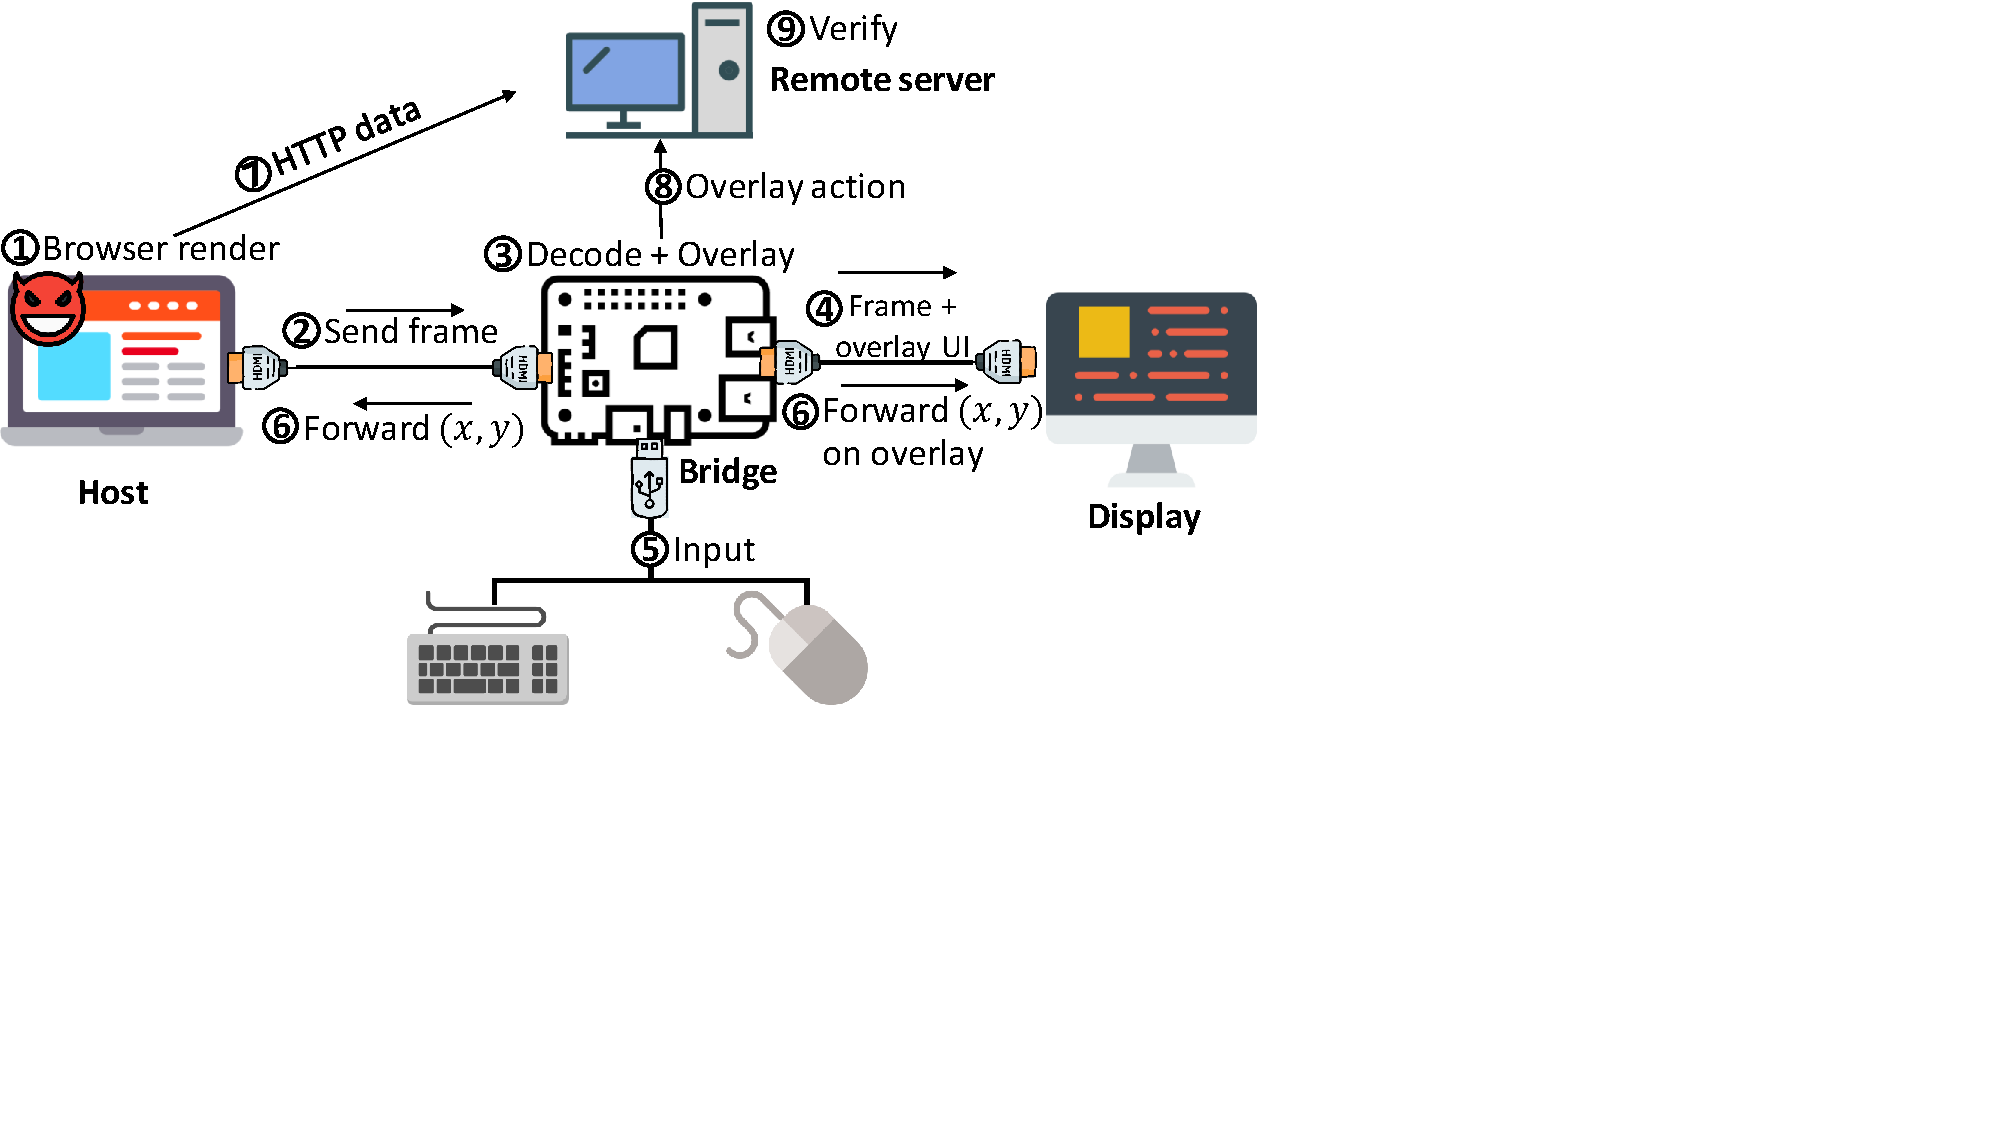
\includegraphics[trim={0 6.5cm 12cm 0}, clip, width=\linewidth]{systemDesign.pdf}
\caption{\textbf{Flow of the \name main protocol.} The figure shows the high-level protocol flow and the main messages that are exchanged between the remote server, host, \device, and the Io devices.}
\spacesave
\label{fig:systemDesign}
\centering
\end{figure}


Now in this Section, we describe the flow of \name protocol by putting these components together. The outline of \name is illustrated in Figure~\ref{fig:systemDesign}. In the flow, we assume that the user already clicked on a web link or typed the URL in the address bar of the browser. This also allows the \device and the remote server to establish a \tls channel using the method described in Section~\ref{sec:confidentiality:tls}. The rest of the steps are the as the following:


\begin{mylist}
  \item[\one] The browser renders the webpage that comes with \name JS. As described in Section~\ref{sec:systemDesign:transformation}, \name JS transforms the UI elements to a QR code that contains the equivalent UI specification.
  \item[\two] The graphics driver sends the rendered frame to the \device over the HDMI channel.
  \item[\three] The \device intercepts the HDMI signal and decode the QR code to retrieve the UI specification. After the decoding of the QR code, the \device renders the bitmap corresponding to the specification as described in Section~\ref{sec:systemDesign:transformation}.
  \item[\four] The \device send the HDMI frame with the UI overlay to the display device.
  \item[\five] After observing the HDMI frame and the overlaid UI, the user passes her input to the \device via the keyboard/mouse that is connected to the \device over the \usb interface.
  \item[\six] The \device uses raw mouse data and the HDMI frames to interpolate the mouse pointer using the method described in Section~\ref{sec:systemDesign:analysis}. This ensures pointer integrity. \device also overlays a mouse pointer on the HDMI frames.
  \item[\seven] When the user input her data to the host, the \device records her input data (Record phase in Section~\ref{sec:systemDesign:commit:send}).
  \item[\eight] The \name JavaScript snippet also acts as a upstream channel from the \device to the remote server (refer to Section~\ref{sec:systemDesign:commit:upload}). Via this channel, the \device sends the signed user action to the remote server. This signed user action can be seen as the second factor for the integrity of the user input data. (Commit phase in Section~\ref{sec:systemDesign:commit:send})
  \item [\nine] The server verifies the data from the two channels that are submitted by the host and the \device. (Section~\ref{sec:systemDesign:commit:verification})
\end{mylist}


\section*{Formal Proof for IO Integrity}
\label{appendix:security}

In this section we provide a formal proof for the security properties of \name. Namely,  without protecting both input and output integrity, none of them can be achieved. To simplify the proof, we model the interaction between the user, the host and the remote server as a final state automate (FSA).

\begin{figure}[h]
\begin{center}
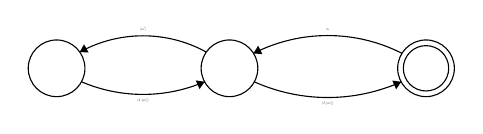
\begin{tikzpicture}[scale=0.15]
\tikzstyle{every node}+=[inner sep=0pt]
\draw [black] (66,-23.1) circle (3);
\draw (66,-23.1) node {\server};
\draw [black] (66,-23.1) circle (2.4);
\draw [black] (45.2,-23.1) circle (3);
\draw (45.2,-23.1) node {\host};
\draw [black] (26.9,-23.1) circle (3);
\draw (26.9,-23.1) node {\user};
\draw [black] (47.743,-21.516) arc (116.95563:63.04437:17.332);
\fill [black] (47.74,-21.52) -- (48.68,-21.6) -- (48.23,-20.71);
\draw (55.6,-19.13) node [above] {$m$};
\draw [black] (29.352,-21.382) arc (118.8302:61.1698:13.89);
\fill [black] (29.35,-21.38) -- (30.29,-21.43) -- (29.81,-20.56);
\draw (36.05,-19.16) node [above] {$[m']$};
\draw [black] (42.565,-24.526) arc (-66.78269:-113.21731:16.527);
\fill [black] (42.57,-24.53) -- (41.63,-24.38) -- (42.03,-25.3);
\draw (36.05,-26.36) node [below] {$(I,[m'])$};
\draw [black] (63.369,-24.535) arc (-65.91058:-114.08942:19.034);
\fill [black] (63.37,-24.53) -- (62.43,-24.4) -- (62.84,-25.32);
\draw (55.6,-26.69) node [below] {$(I,[m'])$};
\end{tikzpicture}
\end{center}
\caption{Finite state machine that depicts the interaction between the user (\user), host (\host) and the server (\server).}
\label{fig:fsm}
\end{figure}

\begin{figure}[h]
\begin{center}
\tikzset{
  every picture/.append style={
    transform shape,
    scale=0.8
  }
 }
\begin{sequencediagram}
\newinst{u}{\user}
\newinst[3]{h}{\host}
\newinst[3]{s}{\server}
\mess{s}{$m$}{h}
\mess{h}{$[m']_1$}{u}
\mess{u}{$I_1,[m']_1$}{h}
%\mess{h}{$[m']_2$}{u}
%\mess{u}{$I_2,[m']_2$}{h}
\mess{h}{...}{u}
\mess{u}{...}{h}
\mess{h}{$[m']_n$}{u}
\mess{u}{$I_n,[m']_n$}{h}
\mess{h}{$I_1,I_2,...,I_n$}{s}
\mess{h}{$[m']_1,[m']_2,...,[m']_n$}{s}
\end{sequencediagram}
\end{center}
\caption{Protocol transcript between the \server, \user and \host that shows one trace from the FSM depicted in Figure~\ref{fig:fsm}.}
\label{fig:protocol}
\end{figure}

\subsection{Interaction Protocol} 
\label{appendix:security:protocol}


The interaction between the server (\server), user (\user) and host (\host) is depicted in the finite state machine in Figure~\ref{fig:fsm}. \server sends a message $m$ to \host. One can assume $m$ to be the HTML, JS send from \server. We denote $[m]$ to be the render of $m$ by the \host. As \host is malicious, it can transform $m$ to $m'$. Note that the transformation is public knowledge and is deterministic. If $m\neq m'$ then given $[m]$ and $[m']$, \server can determine that $[m]\neq [m']$. We denote the user input to be $I$ which corresponds to a specific $[m]$. 
%Note that the communication channel between \server to \user is neither authenticated, neither confidential. But the communication channel from \user and \server is authenticated. 
In this model, we simplify the user input by assuming that the \user only provides an input $I$ only after observing a message transformation $[m]$. The user provides both her input $I$ and transformation $[m']$ observed by her to \host. The interaction loop between \host and \user can continue until \user finishes her input. After every input \host hands over new message transformation to \user (either result of the input or new message from \server or both). Once the user provides all her inputs, \host send the pairs $(I, [m'])$ to \server.

We also define two functions:
\begin{align*}
\texttt{Input()}&:[m]\rightarrow I \\
\texttt{Transform()}&:m,I\rightarrow [m'],\ \exists i\in I:i=\phi
\end{align*}
Both of them are \emph{bijective}.

One trace of the protocol transcript is depicted in Figure~\ref{fig:protocol}. As described in the FSM, \server receives traces of message transformation ($[m']_1,[m']_2,\ldots,[m']_n$) and corresponding inputs ($I_1,I_2,\ldots,I_n$). From these traces \server could determine of all the $[m']_i$ are in proper form by verifying if $[m]_i=[m']_i$.

\begin{definition}{\textbf{Input integrity}}
\label{def:inputIntegrity}
Assume that \server handed a message $m$ to \host where the proper message transformation is $[m]$. The host changes the message transformation to $[m']$ where $[m']\neq [m]$. We also define correct \user input to be $I$ when \host sends a correct message transformation $[m]$ to \user. We define input integrity as the property where the \server does not accept input $I'$ where $I'\neq I$from \user if the \host changes the message transformation.
\end{definition}

\begin{definition}{\textbf{Output integrity}}
\label{def:outputIntegrity}
Assume that \server handed a message $m$ to \host where the proper message transformation is $[m]$. Output integrity defines that in all circumstances, \user receives the correct message transformation $[m]$ from \host.
\end{definition}

\myparagraph{Verification process} \server checks $\forall i=1\ldots n$ $$[m']_i = \texttt{Transform}(m_{i-1}, I_{i-1})$$ where $I_0=\phi$.

\begin{theorem}
\label{theorem:th1}
If \user does not send all the transformations till $[m']_i$ corresponding to the input $I_i$, input integrity can not be achieved. 
\end{theorem}

\begin{IEEEproof}
If \user does not attach all the transformation till $[m']_i$, i.e., $[m']_1, [m']_2, \ldots, [m']_{i-1}, [m']_i$  corresponding to inputs $I_1, I_2,\ldots, I_{i-1}, I_i$, then the server can not verify all the transformations corresponding to the input. \host could modify a specific $[m]_x$ to influence \user input.
\end{IEEEproof}

\begin{theorem}
\label{theorem:th2}
If the channel from \user and \server is not authenticated, input integrity is not achievable. But the channel from \server to \user does not require to be secure as long a \user provides the message transformation $[m']_i$ corresponding to every input $I_i$.
\end{theorem}

\begin{IEEEproof}
The proof is trivial. If the channel from \user to \server is not authenticated, any input provided by \user can be manipulated by \host without a trace. Hence input integrity is not achievable. As long as \user sends message transformation along with the input, a manipulated message transformation bt \host would be detectable by \server (see Theorem~\ref{theorem:th1}).
\end{IEEEproof}

\begin{theorem}
\label{theorem:th3}
Ensuring output integrity also ensures input integrity provided there is an authenticated channel from \user to \server.
\end{theorem}

\begin{IEEEproof}
This proof is also trivial. As we describe in the Definition~\ref{def:inputIntegrity} and~\ref{def:outputIntegrity}, if all the message transform from \host $[m']=[m]$, and \host always executes \texttt{transform()} properly, the input integrity is preserved. As \name ensures output integrity and all the input from the user is signed by the \device, \name preserves input integrity. 
\end{IEEEproof}


